\chapter{Descrizione generale}

\section{Inquadramento}
La piattaforma è stata progettata con lo scopo di erogare dei servizi tipicamente richiesti in ambito aziendale come la gestione delle
informazioni degli utenti, meccanismi di autenticazioni e autorizzazione, l'invio di
email e la sottoscrizione a servizi generici in versione di prova.
L'erogazione di questi servizi avviene grazie ai seguenti elementi (vedi Figura \ref*{fig:Piattaforma}):
\begin{itemize}
    \itemsep0em
    \item Client: applicazione front-end che permette agli utenti di sfruttare le funzionalità della piattaforma inviando delle richieste alla API e mostrando le risposte.
    \item API Web: web Server che permette di gestire le richieste del client e fornisce una interfaccia REST per erogare i servizi.
    \item Microservizio Mailer: servizio interno che gestisce la generazione dei template delle email e l'invio.
    \item Message Broker: permette di fare interagire API Web e il microservizio Mailer.
    \item Email System: sistema esterno utilizzato per l'effettivo invio delle email agli utenti.
    \item Database: permette di gestire i dati in modo permanente.
\end{itemize}

\begin{figure}[h]
    \centering
    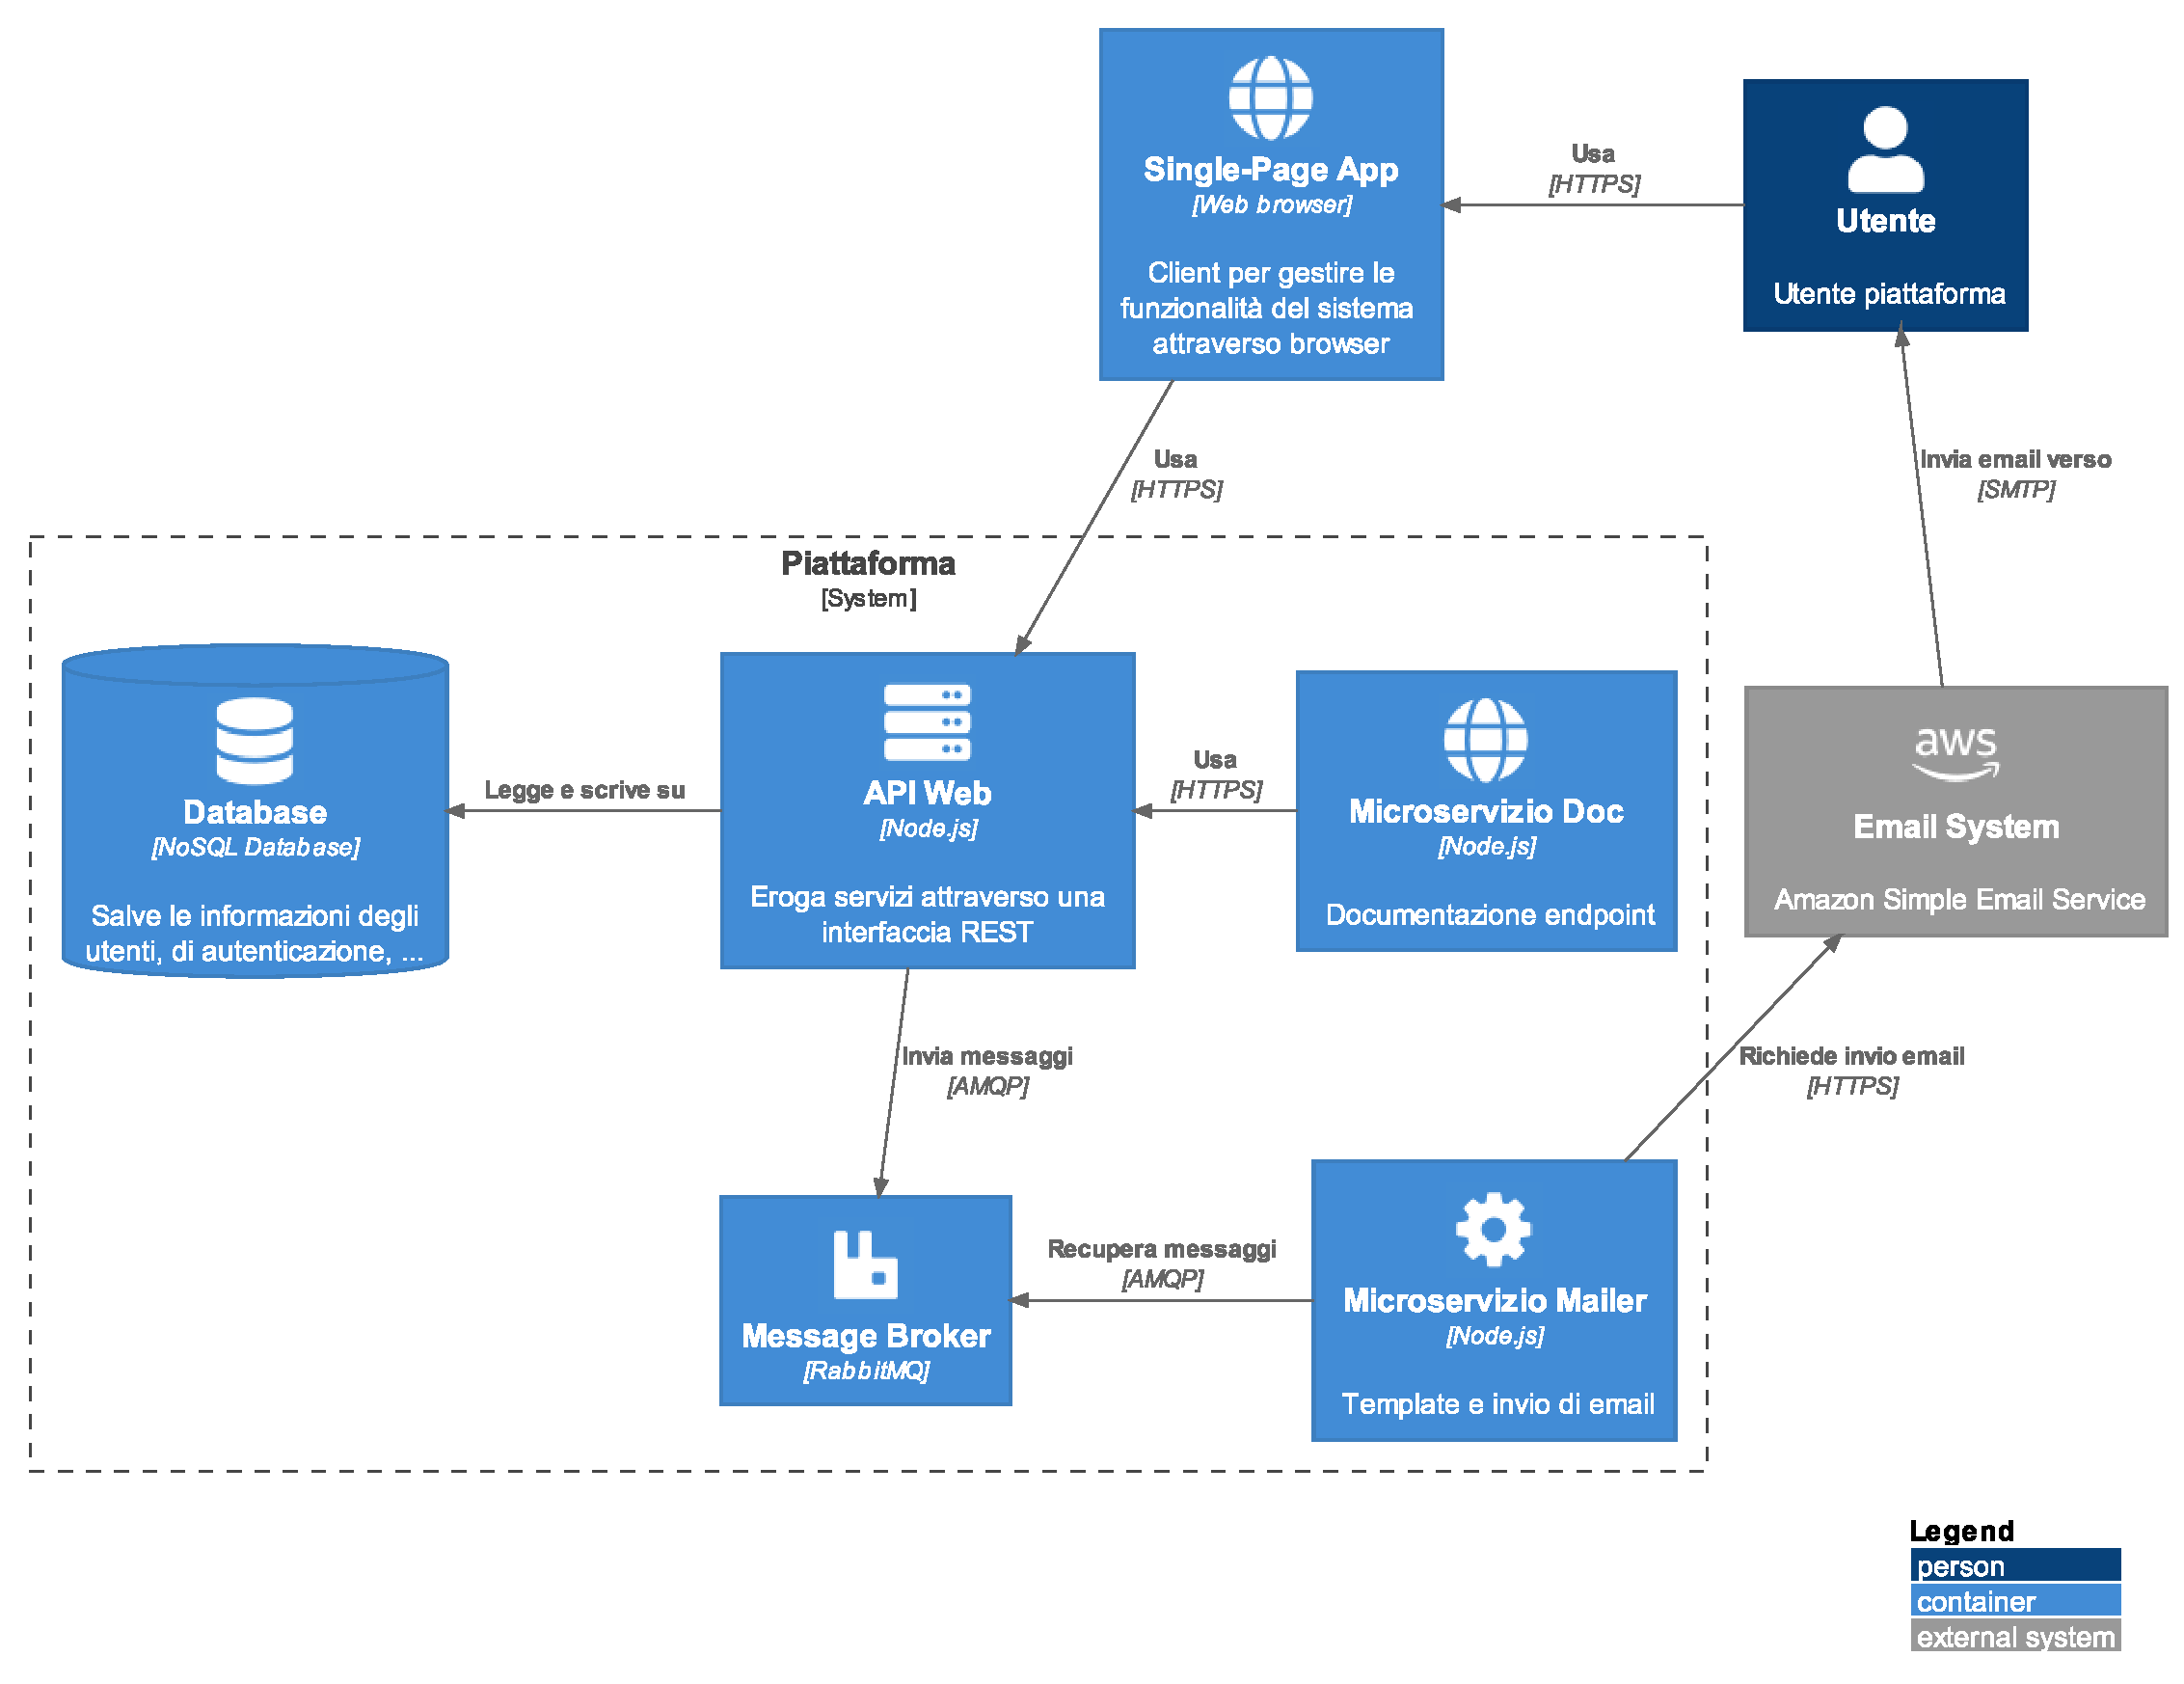
\includegraphics[width=0.8\textwidth]{container-diagram-generale.eps}
    \caption{Architettura piattaforma}
    \label{fig:Piattaforma}
\end{figure}

\section{Macrofunzionalità del sistema}
elenco funzionalità dettagliate

\section{Caratteristiche degli utenti}
utenti normali
admin

\section{Vincoli generali}
Scalabilità
robustezza
sicurezza
collaborazione

